\documentclass[11pt,letterpaper]{article}

\usepackage[utf8]{inputenc}
\usepackage[T1]{fontenc}
% ⚠ lmodern is load-bearing on Linux, not a style choice. tectonic runs XeTeX,
% where `\usepackage[T1]{fontenc}` alone leaves the default font resolving to the
% Latin Modern OPENTYPE face, and on a Linux runner that is not present in the
% bundle:
%   size11.clo:54: Font TU/lmr/m/n/10.95=[lmroman10-regular]:mapping=tex-text
%   not loadable: Metric (TFM) file or installed font not found
% It builds on macOS regardless, which is why this went unnoticed until the repo
% had CI. //deck already carried lmodern and was the only tectonic doc that built.
\usepackage{lmodern}

\usepackage{amsmath,amssymb,amsthm}
\usepackage{microtype}
\usepackage[margin=1in]{geometry}
\usepackage{hyperref}
\usepackage{cleveref}
\usepackage{booktabs}
\usepackage{array}
\usepackage{enumitem}
\usepackage{pgfplots}
\pgfplotsset{compat=1.18}
\usepackage{tikz}
\usetikzlibrary{arrows.meta,positioning,calc,backgrounds}

\hypersetup{colorlinks=true, linkcolor=blue!55!black, citecolor=blue!55!black, urlcolor=blue!55!black}

\theoremstyle{plain}
\newtheorem{theorem}{Theorem}[section]
\newtheorem{proposition}[theorem]{Proposition}
\theoremstyle{definition}
\newtheorem{definition}[theorem]{Definition}

\newcommand{\prior}{\pi_{\mathrm{prior}}}
\newcommand{\Mani}{\mathcal{M}}
\newcommand{\Graphs}{\mathcal{G}}
\newcommand{\Proj}{P}

\title{Crystallization: Spec-Graph Refinement as\\ Training-Free Graph Diffusion}
\author{}
\date{}

\begin{document}
\maketitle

\begin{abstract}
We give a mathematical account of \emph{spec crystallization} --- the process by
which a rough corpus of documents and ideas is refined into a compact, strongly
linked, contradiction-free knowledge graph --- as a \emph{diffusion} process over
typed graphs. The account is deliberately precise about where the analogy to
generative diffusion models is literal and where it is not. We model specifications
as categorical attributed graphs (the state space of discrete graph-diffusion
models), define a forward noising process whose stationary distribution is a
maximum-entropy ``claim gas,'' and target a Gibbs measure
$\pi_\tau(G)\propto e^{-E(G)/\tau}$ induced by an explicit \emph{spec energy}
$E(G)$. Refinement is then a \emph{predictor--corrector} annealed sampler: a
stochastic, training-free language-model predictor proposes graph edits, and a
deterministic, machine-checked projection corrects them onto a gate-passing
manifold without ever raising the energy. We show this alternation makes the
energy a supermartingale, so annealing $\tau\to 0$ concentrates on local minima
--- \emph{crystals}. The resulting object is, precisely, a \emph{training-free,
energy-guided, predictor--corrector graph-diffusion sampler}; it is not a trained
diffusion model, and we say exactly why. We close with what the formalism buys
(an objective, a schedule, a convergence argument) and a path to a genuinely
learned variant.
\end{abstract}

\section{Introduction}
\label{sec:intro}

A specification library is a graph: claims are nodes, and relationships
(\textsf{refines}, \textsf{dependsOn}, \textsf{conflictsWith}, \textsf{realizes})
are typed edges. Authoring such a library at scale is the problem of taking a
high-entropy starting point --- scattered prose, draft ideas, imported standards
--- and \emph{refining} it into something coherent and compact without losing the
thread. This paper argues that the right formal model for that refinement is
\emph{diffusion}, in the precise sense used by modern generative
modeling~\cite{ho2020ddpm,song2021sde,austin2021d3pm,vignac2022digress}.

% Forward (noising) vs reverse (denoising) over typed claim graphs.
\begin{figure}[t]
\centering
\resizebox{\linewidth}{!}{%
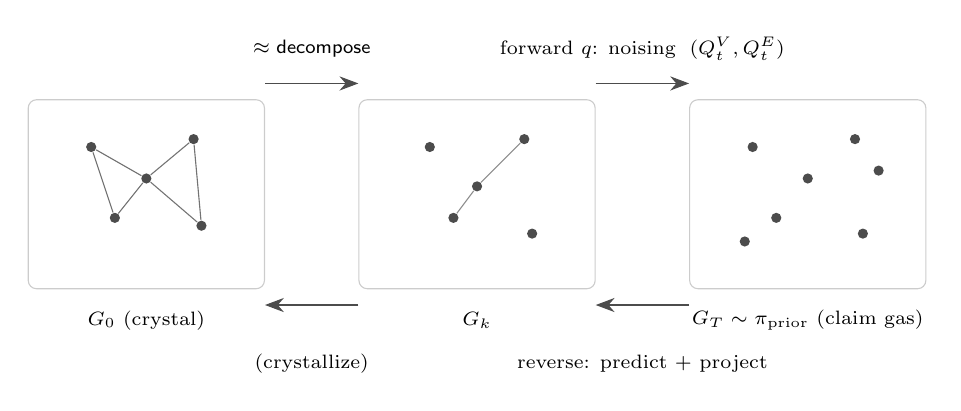
\begin{tikzpicture}[
  font=\footnotesize, >={Stealth[length=2.4mm]},
  cn/.style={circle, fill=black!70, inner sep=1.3pt},
  panel/.style={draw=black!20, rounded corners=3pt, minimum width=30mm, minimum height=24mm},
]
% Panel G0 — coherent crystal (connected, typed)
\node[panel] (p0) at (0,0) {};
\node[font=\scriptsize] at (0,-1.6) {$G_0$ (crystal)};
\node[cn] (a0) at (-0.7,0.6) {}; \node[cn] (b0) at (0.6,0.7) {};
\node[cn] (c0) at (-0.4,-0.3) {}; \node[cn] (d0) at (0.7,-0.4) {};
\node[cn] (e0) at (0.0,0.2) {};
\draw[black!55] (a0)--(e0) (b0)--(e0) (c0)--(e0) (d0)--(e0) (a0)--(c0) (b0)--(d0);

% Panel Gk — partially noised
\node[panel] (pk) at (4.2,0) {};
\node[font=\scriptsize] at (4.2,-1.6) {$G_k$};
\node[cn] at (3.6,0.6) {}; \node[cn] (bk) at (4.8,0.7) {};
\node[cn] (ck) at (3.9,-0.3) {}; \node[cn] at (4.9,-0.5) {};
\node[cn] (ek) at (4.2,0.1) {};
\draw[black!45] (bk)--(ek) (ck)--(ek);

% Panel GT — claim gas (max entropy, edgeless)
\node[panel] (pt) at (8.4,0) {};
\node[font=\scriptsize] at (8.4,-1.6) {$G_T\sim\pi_{\mathrm{prior}}$ (claim gas)};
\foreach \x/\y in {-0.7/0.6, 0.6/0.7, -0.4/-0.3, 0.7/-0.5, 0.0/0.2, 0.9/0.3, -0.8/-0.6}
  {\node[cn] at (8.4+\x,\y) {};}

% Arrows
\draw[->, black!70] ([yshift=2mm]p0.north east) -- ([yshift=2mm]pk.north west)
  node[midway, above, font=\scriptsize] {};
\draw[->, black!70] ([yshift=2mm]pk.north east) -- ([yshift=2mm]pt.north west);
\node[font=\scriptsize] at (6.3,1.85) {forward $q$: noising $\;(Q^V_t,Q^E_t)$};
\node[font=\scriptsize] at (2.1,1.85) {$\approx\textsf{decompose}$};

\draw[->, black!70] ([yshift=-2mm]pt.south west) -- ([yshift=-2mm]pk.south east);
\draw[->, black!70] ([yshift=-2mm]pk.south west) -- ([yshift=-2mm]p0.south east);
\node[font=\scriptsize] at (6.3,-2.15) {reverse: predict $+$ project};
\node[font=\scriptsize] at (2.1,-2.15) {(crystallize)};
\end{tikzpicture}%
}
\caption{Refinement as graph diffusion. The forward process corrupts a coherent
spec graph $G_0$ toward a maximum-entropy ``claim gas'' $\pi_{\mathrm{prior}}$
(type-marginal nodes, no edges); \textsf{decompose} initializes near that prior
directly from a document. The reverse process alternates a stochastic predictor
with a deterministic projection to crystallize a coherent, compact graph.}
\label{fig:diffusion}
\end{figure}


The intuition is that refinement runs a denoising process \emph{backwards} from
disorder to structure (\cref{fig:diffusion}), driven by two cooperating engines:
a \emph{stochastic} one that proposes (large language models, which guess plausible
structure) and a \emph{deterministic} one that disposes (graph algorithms that
provably remove redundancy and contradiction). The contribution of this note is to
make that intuition a definition, to identify which diffusion construct each engine
instantiates, and --- equally important --- to mark honestly where the analogy is
literal and where it is only structural.

\paragraph{Summary of the correspondence.} Specifications live in the categorical
node/edge state space of discrete graph diffusion (\cref{sec:state}); a forward
chain corrupts them toward a tractable prior (\cref{sec:forward}); the ``data
distribution'' is replaced by a Gibbs measure over an explicit energy
(\cref{sec:energy}); the reverse process is Song et al.'s predictor--corrector
sampler, with a language-model predictor and a \emph{proven} projection corrector
(\cref{sec:reverse}); the noise schedule is an annealing temperature and
conditioning is classifier-free guidance (\cref{sec:schedule}); and convergence is
annealed descent to a local minimum we call a crystal (\cref{sec:crystal}).
\Cref{sec:scope} states what may and may not be claimed.

\section{The state space}
\label{sec:state}

\begin{definition}[Spec graph]
A \emph{spec graph} $G=(V,E)\in\Graphs$ is a finite directed graph in which each
node $v\in V$ is a \emph{claim} carrying categorical attributes
$a(v)=(\mathrm{modality},\mathrm{tier},\mathrm{sectionKind},\mathrm{grounding})$,
with $\mathrm{modality}\in\{\textsf{MUST},\textsf{MUST\_NOT},\textsf{SHOULD},
\textsf{SHOULD\_NOT},\textsf{MAY},\textsf{REQUIRED},\textsf{RECOMMENDED}\}$ and
$\mathrm{grounding}\in\{\textsf{grounded},\textsf{loose}\}$; and each ordered pair
$(u,v)$ carries an edge label $e(u,v)\in\mathcal{T}\cup\{\bot\}$, where
$\mathcal{T}$ is a finite set of edge types and $\bot$ denotes ``no edge.''
\end{definition}

This is exactly the categorical node/edge state used by discrete graph-diffusion
models such as DiGress~\cite{vignac2022digress} and the discrete diffusion family
D3PM~\cite{austin2021d3pm}; nodes and edges take values in finite alphabets rather
than in $\mathbb{R}^d$. \emph{This correspondence is literal:} the data type a graph
diffusion operates on and the data type a spec library is are the same.

\section{The forward process and the prior}
\label{sec:forward}

\begin{definition}[Forward noising]
The forward process is a Markov chain with factorized categorical kernels
\[
\begin{aligned}
  q(G_t\mid G_{t-1})=\;&\prod_{v\in V}\mathrm{Cat}\big(a_t(v)\mid a_{t-1}(v)\,Q^V_t\big)\\
  &\times\prod_{(u,v)}\mathrm{Cat}\big(e_t(u,v)\mid e_{t-1}(u,v)\,Q^E_t\big),
\end{aligned}
\]
with row-stochastic transition matrices $Q^V_t,Q^E_t$ whose marginals relax toward
a reference distribution $m$ over attributes and edge types. As in D3PM, the
$t$-step marginal $q(G_t\mid G_0)$ is available in closed form.
\end{definition}

\begin{definition}[Prior]
The \emph{prior} $\prior=\lim_{t\to T}q(G_t\mid G_0)$ is the maximum-entropy
``claim gas'': node attributes drawn i.i.d.\ from $m$, every edge $\bot$, grounding
$\textsf{loose}$. It is tractable to sample and is the analogue of the Gaussian
prior in continuous diffusion.
\end{definition}

In practice one rarely runs this chain on a real document. The \textsf{decompose}
operator maps a narrative or standard directly to a high-entropy seed near
$\prior$ (atomized, loosely linked claims); starting reverse sampling from a
near-prior state is standard. \emph{Honest caveat:} the forward chain is thus a
conceptual device --- and an optional tool for training or stress-testing the
corrector by corrupting known-good graphs --- not a daily-run component.

\section{Energy and the Gibbs target}
\label{sec:energy}

The role played by the (unknown) data distribution $p_0$ in generative diffusion
is played here by a Gibbs measure over an \emph{explicit, computable} energy.

\begin{definition}[Spec energy]
\label{def:energy}
For weights $w_i>0$,
\[
  E(G)=w_1 R(G)+w_2 C(G)+w_3 D(G)+w_4 U(G)-w_5 L(G)-w_6 S(G),
\]
where $R$ is redundancy (duplicated claims/edges), $C$ is contradiction count,
$D$ is dangling/loose references, $U$ is under-specification (the frontier), $L$ is
meaningful connectivity, and $S$ is symmetry compression (the description-length
saving from collapsing isomorphic sub-graphs). Each term is computable by query
over the graph.
\end{definition}

\begin{definition}[Target]
The target distribution at temperature $\tau$ is the Boltzmann measure
$\pi_\tau(G)\propto e^{-E(G)/\tau}$. Its low-energy support is the ``manifold of
coherent specifications.''
\end{definition}

On a discrete space the analogue of the Stein score $\nabla_x\log p_t(x)$ is the
collection of local conditional ratios $\pi_\tau(G')/\pi_\tau(G)$ over neighbors
$G'$ of $G$; an edit that lowers $E$ is a discrete score-ascent step, in the sense
made precise by discrete diffusion~\cite{austin2021d3pm}. \emph{Honest caveat:}
unlike a learned diffusion model, whose score implicitly defines the data manifold,
our manifold is \emph{axiomatized} by $E$ and the gates of \cref{sec:reverse}. The
strength is that it is inspectable and partly machine-checked; the limitation is
that result quality is bounded by the quality of $E$.

\section{Reverse dynamics: predictor--corrector}
\label{sec:reverse}

We instantiate the reverse (denoising) process as the predictor--corrector sampler
of Song et al.~\cite{song2021sde}: a step that moves toward the target, followed by
steps that re-equilibrate to it.

% The predictor-corrector refinement step.
\begin{figure}[t]
\centering
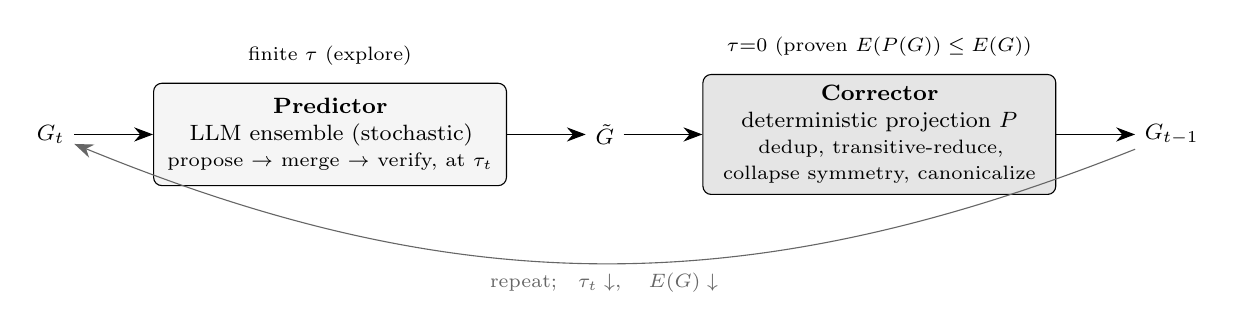
\begin{tikzpicture}[
  font=\footnotesize, >={Stealth[length=2.4mm]}, node distance=10mm,
  box/.style={draw, rounded corners=3pt, align=center, minimum height=13mm,
              text width=42mm, inner sep=4pt},
  pred/.style={box, fill=black!4},
  corr/.style={box, fill=black!10},
  st/.style={font=\footnotesize},
]
\node[st] (gt) {$G_t$};
\node[pred, right=of gt] (P) {\textbf{Predictor}\\ LLM ensemble (stochastic)\\ \scriptsize propose $\to$ merge $\to$ verify, at $\tau_t$};
\node[st, right=of P] (gm) {$\tilde G$};
\node[corr, right=of gm] (C) {\textbf{Corrector}\\ deterministic projection $P$\\ \scriptsize dedup, transitive-reduce, collapse symmetry, canonicalize};
\node[st, right=of C] (gt1) {$G_{t-1}$};

\draw[->] (gt) -- (P);
\draw[->] (P) -- (gm);
\draw[->] (gm) -- (C);
\draw[->] (C) -- (gt1);
\draw[->, black!60] (gt1) to[bend left=22]
  node[below, font=\scriptsize] {repeat; \; $\tau_t\downarrow$, \;\; $E(G)\downarrow$} (gt);

\node[font=\scriptsize, align=center, above=1mm of P] {finite $\tau$ (explore)};
\node[font=\scriptsize, align=center, above=1mm of C] {$\tau{=}0$ (proven $E(P(G))\le E(G)$)};
\end{tikzpicture}
\caption{One reverse step is \emph{predict then project}. The predictor is a
training-free, in-context LLM denoiser exploring at temperature $\tau_t$; the
corrector is a deterministic, machine-checked projection onto the gate-passing
manifold that never raises the energy. Iterating with $\tau_t\to 0$ crystallizes
the graph.}
\label{fig:pc}
\end{figure}


\paragraph{Predictor (stochastic).} Given the current graph $G_t$, an ensemble of
language models proposes a cleaner graph $\tilde G$ --- predicting claim types,
groundings, and edges from the noisy neighborhood, conditioned on the guiding
vision (\cref{sec:schedule}). This is a \emph{training-free, in-context} denoiser:
a pretrained model used zero/few-shot, \emph{not} a network trained by denoising
score matching. \emph{This is the central place the analogy is structural rather
than literal} (\cref{sec:scope}).

\paragraph{Corrector (deterministic).} A projection $\Proj$ applies exact graph
passes --- content-hash deduplication, transitive reduction, symmetry/orbit
collapse, and canonicalization --- onto the gate-passing manifold
$\Mani=\{G:\text{all gates pass}\}$. We require $\Proj$ to satisfy the invariants
\begin{equation}
\label{eq:proj}
  \Proj(G)\in\Mani,\qquad \Proj(\Proj(G))=\Proj(G),\qquad E(\Proj(G))\le E(G),
\end{equation}
together with a meaning-preservation homomorphism $G\to\Proj(G)$ modulo collapsed
symmetry. These invariants are the projection's specification and are intended to
be machine-checked (the deterministic counterpart of a verified arithmetic
kernel). Because each corrector pass cannot raise $E$, corrector moves are
zero-temperature steps that are always accepted.

\begin{definition}[Refinement step]
One reverse step is $G_{t-1}=\Proj\big(\mathsf{Pred}_{\tau_t}(G_t)\big)$ ---
\emph{predict, then project}.
\end{definition}

\section{Schedule and guidance}
\label{sec:schedule}

\paragraph{Schedule.} The temperature $\tau_t:T\to 0$ is the noise schedule:
high early (broad exploration; many cheap parallel predictor trajectories) and low
late (sharpening; expensive high-precision proposals, then deterministic
projection). This is the direct analogue of the $\beta_t$ schedule of
DDPM~\cite{ho2020ddpm}.

\paragraph{Guidance.} A guiding vision $y$ (the intended product space) and a
grounding vocabulary enter as an additional energy term, giving the conditional
target
\[
  \pi_\tau(G\mid y)\propto\exp\!\Big(-\tfrac{1}{\tau}\big(E(G)+\lambda\,E_{\mathrm{cond}}(G,y)\big)\Big),
\]
with the predictor prompted on $y$ (a conditional denoiser) and $\lambda$ the
guidance weight. Structurally this is classifier-free
guidance~\cite{ho2022cfg}: a base score plus a conditioning gradient.

\section{Crystallization (convergence)}
\label{sec:crystal}

% Energy landscape + annealed descent to a crystal (local minimum).
\begin{figure}[t]
\centering
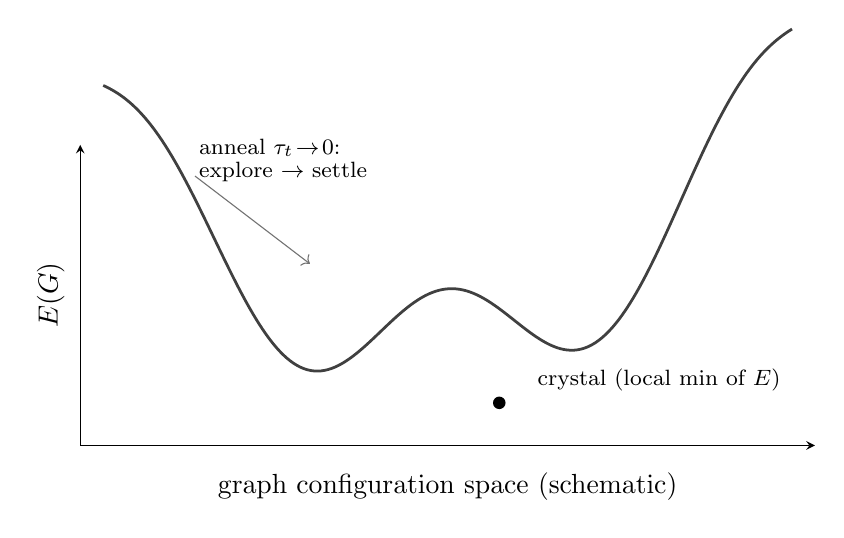
\begin{tikzpicture}
\begin{axis}[
  width=0.9\linewidth, height=5.4cm,
  xlabel={graph configuration space (schematic)},
  ylabel={$E(G)$},
  xmin=-3.2, xmax=3.2, ymin=-1.6, ymax=3.2,
  xtick=\empty, ytick=\empty,
  axis lines=left, every axis x label/.style={at={(axis description cs:0.5,-0.06)},anchor=north},
  clip=false,
]
% A bumpy energy curve with several wells.
\addplot[black!75, line width=1pt, samples=200, domain=-3:3]
  {0.45*x*x + 0.9*cos(deg(2.4*x)) + 0.15*x};
% Mark a local minimum near x = 0.45 (a "crystal").
\node[circle, fill=black, inner sep=1.6pt] (cryst) at (axis cs:0.45,-0.92) {};
\node[anchor=west, font=\footnotesize] at (axis cs:0.7,-0.55) {crystal (local min of $E$)};
% Annealing annotation.
\draw[->, black!55] (axis cs:-2.2,2.7) -- (axis cs:-1.2,1.3);
\node[anchor=west, font=\footnotesize, align=left] at (axis cs:-2.25,2.95)
  {anneal $\tau_t\!\to\!0$:\\[-1pt] explore $\to$ settle};
\end{axis}
\end{tikzpicture}
\caption{Crystallization as annealed descent. At high temperature the sampler
explores broadly; as $\tau_t\to 0$ it concentrates on a local minimum of the
energy $E$ within the gate-passing manifold --- a \emph{crystal}: a fixed point
where the projection is idempotent and no accepted move lowers $E$. As in
practical diffusion, the guarantee is local, not global.}
\label{fig:landscape}
\end{figure}


We accept a predictor proposal $G\to G'$ iff $\Delta E=E(G')-E(G)\le 0$, or with
Metropolis probability $\min\{1,e^{-\Delta E/\tau_t}\}$; corrector moves are always
accepted by \eqref{eq:proj}.

\begin{definition}[Crystal]
A \emph{crystal} is a fixed point $G^\star$ with $\Proj(G^\star)=G^\star$ and no
accepted move that lowers $E$.
\end{definition}

\begin{theorem}[Annealed descent to a crystal]
\label{thm:crystal}
Under the acceptance rule above, the sequence $E(G_t)$ is a supermartingale and
converges almost surely. If, in addition, $\tau_t\to 0$ and every state communicates
with a lower-energy state until a fixed point is reached, the chain converges almost
surely to a crystal, i.e.\ a local minimum of $E$ within $\Mani$.
\end{theorem}

\begin{proof}[Proof sketch]
Corrector moves give $\Delta E\le 0$ deterministically \eqref{eq:proj}. Predictor
moves are Metropolis steps reversible with respect to $\pi_{\tau_t}$, so their
conditional expectation of $E$ is non-increasing in the small-step limit; hence
$\mathbb{E}[E(G_{t+1})\mid G_t]\le E(G_t)$ and $E(G_t)$ is a bounded-below
supermartingale, which converges a.s. As $\tau_t\to 0$ the Metropolis acceptance of
uphill moves vanishes, so the only surviving transitions are downhill or onto the
fixed set; the limit is therefore a state from which no accepted move lowers $E$
and on which $\Proj$ is idempotent --- a crystal.
\end{proof}

\emph{Honest caveat:} the guarantee is \emph{local}, not global. This is the same
situation as practical diffusion sampling, which does not provably reach the global
mode either; the value is a principled stopping criterion and a monotone-progress
argument, not a global optimality claim.

\section{Correspondence and scope}
\label{sec:scope}

\Cref{tab:corr} lays out the mapping and its fidelity.

\begin{table}[t]
\centering
\small
\renewcommand{\arraystretch}{1.18}
\begin{tabular}{@{}p{0.40\linewidth} p{0.40\linewidth} l@{}}
\toprule
\textbf{Generative diffusion} & \textbf{Spec crystallization} & \textbf{Fidelity} \\
\midrule
Categorical node/edge state (DiGress, D3PM) & typed claim/edge graph $\Graphs$ & literal \\
Forward SDE / categorical corruption & $q(G_t\mid G_{t-1})$ via $Q^V_t,Q^E_t$ & literal; rarely run \\
Gaussian / marginal prior $p_T$ & max-entropy claim gas $\prior$ & literal \\
Data distribution $p_0$ & Gibbs $\pi_0\propto e^{-E/\tau_0}$ & analogical \\
Score $\nabla\log p_t$ & local conditional ratios of $\pi_\tau$ & literal (discrete) \\
Learned denoiser $\epsilon_\theta$ & LLM ensemble (in-context) & \textbf{analogical} \\
Predictor step & LLM propose/merge/verify & literal \\
Corrector (Langevin) step & deterministic projection $\Proj$ & literal (proven) \\
Noise schedule $\beta_t$ & temperature $\tau_t$ & literal \\
Classifier-free guidance & vision energy $E_{\mathrm{cond}}$, weight $\lambda$ & literal \\
A generated sample & a crystallized spec graph & literal \\
\bottomrule
\end{tabular}
\caption{The correspondence and its honest fidelity. The single analogical link
that matters is the denoiser: ours is training-free, not score-matched.}
\label{tab:corr}
\end{table}

\paragraph{What may be claimed.} The process is precisely a \emph{training-free,
energy-guided, predictor--corrector annealed graph-diffusion sampler}: the LLM
ensemble is the reverse-process predictor, the proven projection is the corrector,
the temperature is the noise schedule, and crystallization is annealed descent to a
local minimum of an explicit energy on a gate-passing manifold.

\paragraph{What may not be claimed.} It is \emph{not} a trained diffusion model:
there is no score matching and no learned $\epsilon_\theta$; the ``data manifold''
is axiomatized by $E$ and gates rather than learned from a corpus of exemplary
specifications; and convergence is local, not global. Using the term ``diffusion''
without these qualifications would overstate the result.

\section{What the formalism buys, and a path to a learned model}
\label{sec:buys}

\begin{enumerate}[leftmargin=1.4em,itemsep=2pt]
  \item \textbf{An objective.} $E(G)$ makes ``a better specification'' measurable
  and gives refinement a stopping criterion (a crystal).
  \item \textbf{A schedule.} Annealing prescribes where to spend cheap broad
  exploration versus expensive precise proposals, and when to stop.
  \item \textbf{A correctness account.} The corrector's proven monotonicity
  \eqref{eq:proj} is exactly why many parallel stochastic agents \emph{converge}
  rather than thrash: every agent's contribution is filtered through a projection
  that cannot increase disorder.
  \item \textbf{A research path.} Collecting (corrupted, clean) graph pairs via the
  forward process of \cref{sec:forward} would let one train an actual graph
  denoiser $\epsilon_\theta$ and/or an energy $E_\theta$, upgrading the
  training-free sampler into a learned graph-diffusion model. The architecture is
  forward-compatible with that step; nothing above forecloses it.
\end{enumerate}

\begin{thebibliography}{9}
\bibitem{ho2020ddpm} J.~Ho, A.~Jain, P.~Abbeel.
  \newblock Denoising diffusion probabilistic models.
  \newblock In {\em NeurIPS}, 2020.
\bibitem{song2021sde} Y.~Song, J.~Sohl-Dickstein, D.~P. Kingma, A.~Kumar,
  S.~Ermon, B.~Poole.
  \newblock Score-based generative modeling through stochastic differential
  equations.
  \newblock In {\em ICLR}, 2021.
\bibitem{austin2021d3pm} J.~Austin, D.~Johnson, J.~Ho, D.~Tarlow,
  R.~van den Berg.
  \newblock Structured denoising diffusion models in discrete state-spaces (D3PM).
  \newblock In {\em NeurIPS}, 2021.
\bibitem{vignac2022digress} C.~Vignac, I.~Krawczuk, A.~Siraudin, B.~Wang,
  V.~Cevher, P.~Frossard.
  \newblock {DiGress}: Discrete denoising diffusion for graph generation.
  \newblock In {\em ICLR}, 2023.
\bibitem{ho2022cfg} J.~Ho, T.~Salimans.
  \newblock Classifier-free diffusion guidance.
  \newblock In {\em NeurIPS Workshop}, 2021.
\end{thebibliography}

\end{document}
